\chapter{Introduzione}
\label{ch:Introduzione}

\begin{citazione}
Non esiste alternativa alla trasformazione digitale. Le aziende visionarie si ritaglieranno nuove opzioni strategiche, quelle che non si adatteranno falliranno. Jeff Bezos \cite{jeff_bezos_cite}
\end{citazione}

Ormai da anni il mondo ha inglobato nel proprio essere la tecnologia, rendendola parte di esso e in alcuni casi anche imprescindibile. L’evoluzione della tecnologia ha contribuito esponenzialmente alla produzione di nuovi sistemi che migliorassero la vita delle persone, con automazioni e semplificazioni dei normali compiti tediosi o stancanti. Tale evoluzione ha comportato una sempre più importante evoluzione delle infrastrutture atte a permettere la creazione di tali sistemi e soprattutto di un ambiente interconnesso. Proprio per questo motivo, al giorno d'oggi molto spesso si da per scontato la tecnologia e la sua interazione con il mondo. Tuttavia, ciò non va sottovalutato, l'avvento della tecnologia fin dal primo istante ha comportato l'evoluzione del mondo intero dovuto alla necessità di adattamento a quest'ultima. Con il tempo ogni persona ha fatto parte di questo processo, utilizzando tale innovazione e migliorando il proprio stile di vita. Naturalmente, tale evoluzione ha condizionato anche il mondo aziendale, prendendo il nome di \textbf{trasformazione digitale}; più precisamente questa pratica corrisponde al processo di evoluzione dei modelli aziendali, basato sugli avanzamenti tecnologici. Consiste in un cambiamento radicale attuato mediante strumenti digitali ~\cite{redhat_digital_transformation}.

\section{Trasformazione Digitale}
Lo sviluppo economico deriva molto spesso da diversi cambiamenti sociali avvenuti nel tempo. La \textit{trasformazione digitale} (o \textit{digital tranformation, DT}) è uno degli esempi più importanti e recenti che manifestano tale cambiamento. Proprio per questo motivo, molti ricercatori hanno studiato approfonditamente questo fenomeno in modo da poterne identificare le possibili implicazioni, vantaggi, svantaggi e conseguenze sulle pratiche sociali e lavorative. Tutto allo scopo di sfruttare al massimo tale processo in modo da farlo diventare un importante punto fondamentale che permetta di migliorare ulteriormente ~\cite{sciencedirect_digital_transformation}.

Secondo uno studio svolto nel 2018 è stato previsto che durante lo stesso anno sarebbero stati investiti circa 1,3 miliardi di dollari da parte delle aziende per applicare tecniche digitali in modo da incrementare l'efficienza, aumentare il valore del cliente e creare nuove opportunità di monetizzazione. Tuttavia, tale trasformazione non è affatto un compito semplice; infatti, il 70\% di questi processi non è riuscita o riuscirà nel proprio intento, comportando  una perdita totale di oltre 900 milioni di dollari ~\cite{forbes_digital_transformation_fail}.

\subsection{Strategie della trasformazione digitale}

A seguito di approfonditi studi e dell'incremento dell'interesse in questo mondo, molte aziende negli ultimi anni hanno intrapreso un processo di esplorazione e innovazione adoperando nuove tecnologie digitali così da poterne sfruttare i benefici. Ciò ha comportato la necessità di svolgere procedimenti atti a trasformare anche le principali operazioni svolte dalle aziende in questione. Però, per svolgere tale procedura è necessario formulare una strategia di trasformazione corretta e coordinata ~\cite{digital_transformation_strategies}.

\subsection{Benefici}

La maggior parte dei benefici della trasformazione digitale nell'ambito professionale possono essere suddivisi in cinque differenti gruppi ~\cite{sciencedirect_digital_transformation_benefits}:
\begin{itemize}
    \item Miglioramento della produttività: i processi di sviluppo e progettazione hanno diminuito le relative tempistiche necessarie per essere eseguiti.
    \item Incremento della qualità: tramite apposite misurazioni ad alta precisione dei parametri di produzione e dei prodotti durante l'interno processo di produzione è possibile comprendere al meglio tutte le sue fasi, così da conoscere su quale di questi svolgere delle azioni che comportino un risparmio.
    \item Maggiore personalizzazione dei prodotti: svolgendo analisi sui dati rispetto alle interazioni con gli utenti e ulteriori analisi di mercato è possibile comprendere quale siano le preferenze del proprio pubblico.
    \item Aumento della sicurezza: naturalmente l’evoluzione digitale porta non solo migliorie in ambito economico, ma anche in quello della sicurezza del singolo utente che, grazie a nuovi strumenti e metodologie, può svolgere in maggiore sicurezza (o magari non farlo proprio) compiti pericolosi, venendo preventivamente avvisato di potenziali rischi e sulle possibili contromisure.
\end{itemize}

\section{Incremento dei dati}

Sicuramente, tra i vari processi di trasformazione digitale, il principale è stato quello di dematerializzazione dei documenti cartacei, che prende il nome di \textbf{digitalizzazione} (o \textit{digitalization}). Più precisamente quando si parla di digitalizzazione si parla del processo di trasformazione di un'immagine, di un suono, di un documento in un formato digitale, interpretabile da un computer ~\cite{wikipedia_digitalization_definition}.

A seguito di tale processo, le informazioni nel formato digitale, che in precedenza non era stato nemmeno immaginato, hanno acquisito sempre più importanza nel mondo con il nome di \textit{dati} fino a diventare uno, se non il valore più importante.

Lo scopo di tale progetto era riorganizzare la conoscenza in modo sempre più efficiente semplificando la selezione delle notizie in un mondo sommerso dalle informazioni. Fu compreso fin dal primo istante quanto questo fosse ambizioso, tuttavia, forse in parte venne sottostimato quale potesse essere la portata di tale rivoluzione. Tale idea ha portato non solo alla ridistribuzione e organizzazione delle informazioni pregresse, ma anche alla creazione di nuove informazioni dovute proprio a tale processo di modernizzazione. A queste, si sono poi aggiunte sempre più dati da dover salvare e gestire con l'incremento delle nuove tecnologie messe a disposizione dal progresso evolutivo che il mondo stava e sta tutt'ora affrontando. 

\subsection{La Digital DataSphere}

L'azienda IDC \footnote{La \textit{International Data Corporation} (\textit{IDC}) è un fornitore globale di informazioni di mercato, servizi di consulenza ed eventi per i mercati della tecnologia dell'informazione, delle telecomunicazioni e della tecnologia di consumo.} ha localizzato e definito i tre principali ambienti dove la digitalizzazione avviene di continuo e dove tali dati vengono salvati, ovvero:~\cite{idc_digital_datasphere}

\begin{enumerate}
    \item \textit{Core} (o “nucleo”): consiste nei datacenter tradizionali e cloud messi a disposizione dai provider;
    \item \textit{Edge} (o “bordo”): ovvero le infrastrutture delle imprese/aziende che non fanno parte dei datacenter principali; 
    \item \textit{Endpoint} (o “estremo”): con il termine "endpoint" si fa riferimento a tutti i dispositivi personali che sono agli estremi della rete, come PC, smartphone, dispositivi IoT, eccetera. 
\end{enumerate}

\begin{figure}[!h]
    \centering
    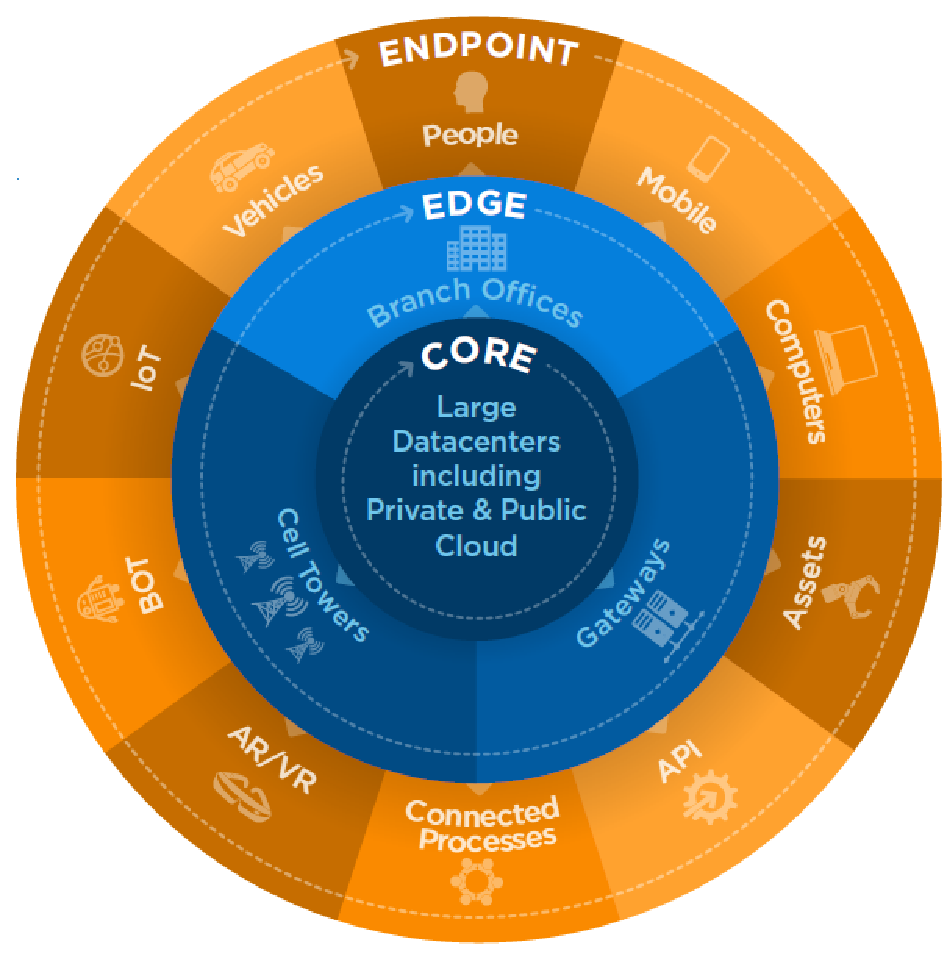
\includegraphics[width=0.3\linewidth]{figure/capitolo_1/Digital-Datasphere.pdf}
    \caption{Digital DataSphere}
    \label{fig:Digital-Datasphere}
\end{figure}

La somma di tutti questi dati forma ciò che loro definiscono come \textbf{Global DataSphere}; più precisamente la Global DataSphere quantifica ed analizza l'ammontare dei dati creati, recuperati e duplicati in un dato anno nell'intero mondo.~\cite{datadrivendaily_dimension_table}

Secondo uno studio del 2018 svolto sull'incremento di tale Global DataSphere~\cite{idc_global_datasphere}, la IDC ha denotato un andamento al quanto impressionante di tipo esponenziale, ovvero secondo le stime entro il 2025 l'ammontare dei dati generati nell'intero mondo sarà pari a 175 Zettabyte (\textit{ZB}, ovvero 270 bit) rispetto ai “soli” 80 del 2022. Leggendo il grafico riportato di seguito, è possibile notare che nel triennio 2023-2025 è stata stimato l'ammontare di 430 Zettabyte di dati, mentre andando dal 2022 a ritroso l'ammontare totale è minore di 400; in altre parole, i dati dell'ultimo triennio superano il totale dei dati creati fino al 2022 dall'inizio della storia della digitalizzazione. Per poter comprendere meglio e farsi un'ieda di quanto questo valore sia elevato, riporto qui un esempio: se volessimo scaricare l'intero DataSphere del 2025, ovvero 175 ZB di dati, con una connessione di 100 Mb/s \footnote{Il valore preso in esempio è stato ricavato facendo riferimento alla media italiana di velocità di download, verificata nel 2022 ~\cite{github_speed_connection}, e poi approssimato per semplicità di calcolo} sarebbero necessari 554.552.923 anni (o più “semplicemente” 5.545.529 secoli) per completare l'operazione.

\begin{figure}[!h]
    \centering
    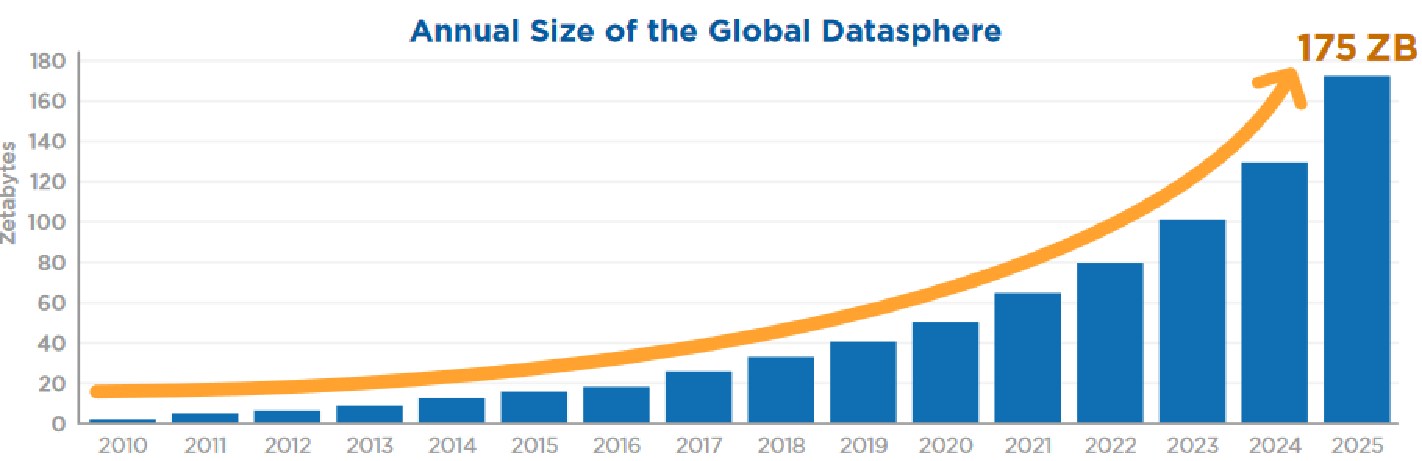
\includegraphics[width=1\linewidth]{figure/capitolo_1/Annual Size Global Datasphere.pdf}
    \caption{Dimensione annuale della Digital Datasphere globale}
    \label{fig:Annual Size Global Datasphere}
\end{figure}

\subsection{Salvataggio e gestione dei dati}

Naturalmente, come è possibile dedurre autonomamente, questo incremento della generazione dei dati è dovuto a multipli fattori, su tutti sicuramente l'aumento di dispositivi a disposizione per la generazione di tali dati e l'espansione nel mondo dell'Internet e del Web con tutti i relativi servizi annessi. Attualmente siamo in un'era dove l'immensa quantità di dispositivi a nostra disposizione danno la possibilità alle persone di eseguire un'enorme quantità di azioni e interazioni, che non fanno altro che generare ulteriori dati e informazioni. L'incremento di tali dati ha generato in questo modo anche la necessità di salvarli e gestirli. Lo storage dei dati è la raccolta e la conservazione di informazioni digitali, tale processo svolge un ruolo sempre più centrale nella gestione dei dati e dei Big Data.~\cite{redhat_data_storage}

Più precisamente quando si parla di gestione dei dati si riferisce al processo di acquisizione, archiviazione e utilizzo dei dati che consente di sapere quali dati sono disponibili, dove si trovano, chi ne è il proprietario, chi può vederli e chi vi può accedere. La gestione dei dati consente alle organizzazioni di eseguire il deployment delle applicazioni e dei sistemi critici in modo sicuro e conveniente e di facilitare le decisioni strategiche.~\cite{redhat_data_management}

\section{Data-Driven Orientation}

Un aspetto molto importante ma che purtroppo viene molto sottovalutato all'interno delle aziende è la conoscenza reale del dato ancora prima della sua fruizione. Questo poiché non è possibile estrapolare informazioni da dati che si hanno a disposizione se non si ha una idea chiara su cosa essi possano effettivamente indicare e valorizzare. Proprio per sopperire a tale problematica, ormai l'approccio \textit{data-driven}, o \textit{data oriented}, è diventato sempre più comune nella maggior parte delle aziende.

\subsection{Il processo decisionale basato sui dati}

La strategia di effettuare delle decisioni basate sui dati è stata introdotta per puntualizzare la necessità di questo nuovo orientamento che considera la raccolta dei dati come un punto cardine delle strategie aziendali. L'adozione di un insieme integrato di tecnologie apposite per l'analisi dei dati può contribuire a facilitare la comunicazione in tempo reale, coinvolgere gli attori nella presa di decisioni e consentire la costante ridefinizione delle interazioni tra gli utenti e la tecnologia così da migliorare il benessere ed ottenere, con l'avanzare del tempo, innovazione e resilienza.~\cite{emerald_data_driven_orientation}

Più precisamente, il \textit{processo decisionale basato sui dati} (\textit{data-driven decision making, DDDM}) si definisce come l'utilizzo di elementi concreti, metriche e dati per orientare il processo decisionale aziendale in linea con obiettivi, scopi e iniziative. Cambiare il modo in cui la tua azienda prende decisioni non è semplice, ma incorporare dati e analisi nei cicli decisionali è il modo più efficace per generare il massimo dell'evoluzione dell'organizzazione. Proprio per questo motivo, per un'organizzazione è necessario rendere il processo decisionale data-driven una prassi.~\cite{tableau_data_driven_decision_making}

\subsection{Punti chiave delle aziende data-driven}
Le aziende data-driven basano la loro organizzazione su cinque punti chiave:~\cite{researchgate_data_driven_orientation}

\begin{enumerate}
    \item \textit{Digital transformation}. Per poter integrare i dati all'interno dei processi decisionali è necessario che questi siano naturalmente presenti e disponibili. Per permettere ciò è necessaria una chiara strategia di trasformazione digitale.
    \item \textit{Data science}. Con l'avvento dell'adozione di strumenti tecnologici, il modo in cui le organizzazioni producono, condividono e sfruttano i dati è cambiato. Per tale motivo la Data Science (è lo studio dei dati per estrarre informazioni significative per il business ) ha trovato nuovi modi per analizzare e ottenere valore dai dati.
    \item \textit{Data-Driven business model}. Al fine di generare ulteriore valore economico, le intuizioni aziendali acquisite devono essere sfruttate all'interno dei modelli di business. Una parte cruciale di questo processo è proprio la creazione di valore dalle informazioni digitalizzate, definendo come un DDBM si basi principalmente sul vedere i dati come una risorsa economicamente importante su cui investire.
    \item \textit{Data-Driven innovation}. Le aziende utilizzano i dati, da loro generati e raccolti, per trasformare le loro attività commerciali in innovazioni basate su questi. Attraverso tale innovazione, le organizzazioni sono abilitate ad utilizzare, e gestire coerentemente, le loro enormi quantità di dati (Big Data).
    \item \textit{Data Analytics}. Il valore dei dati ricercato deriva da un'attenta, corretta e congruente analisi dei dati a disposizione. Tale analisi permette alle compagnie di incrementare al meglio le proprie conoscenze aziendali.
\end{enumerate}

\begin{figure}[!h]
    \centering
    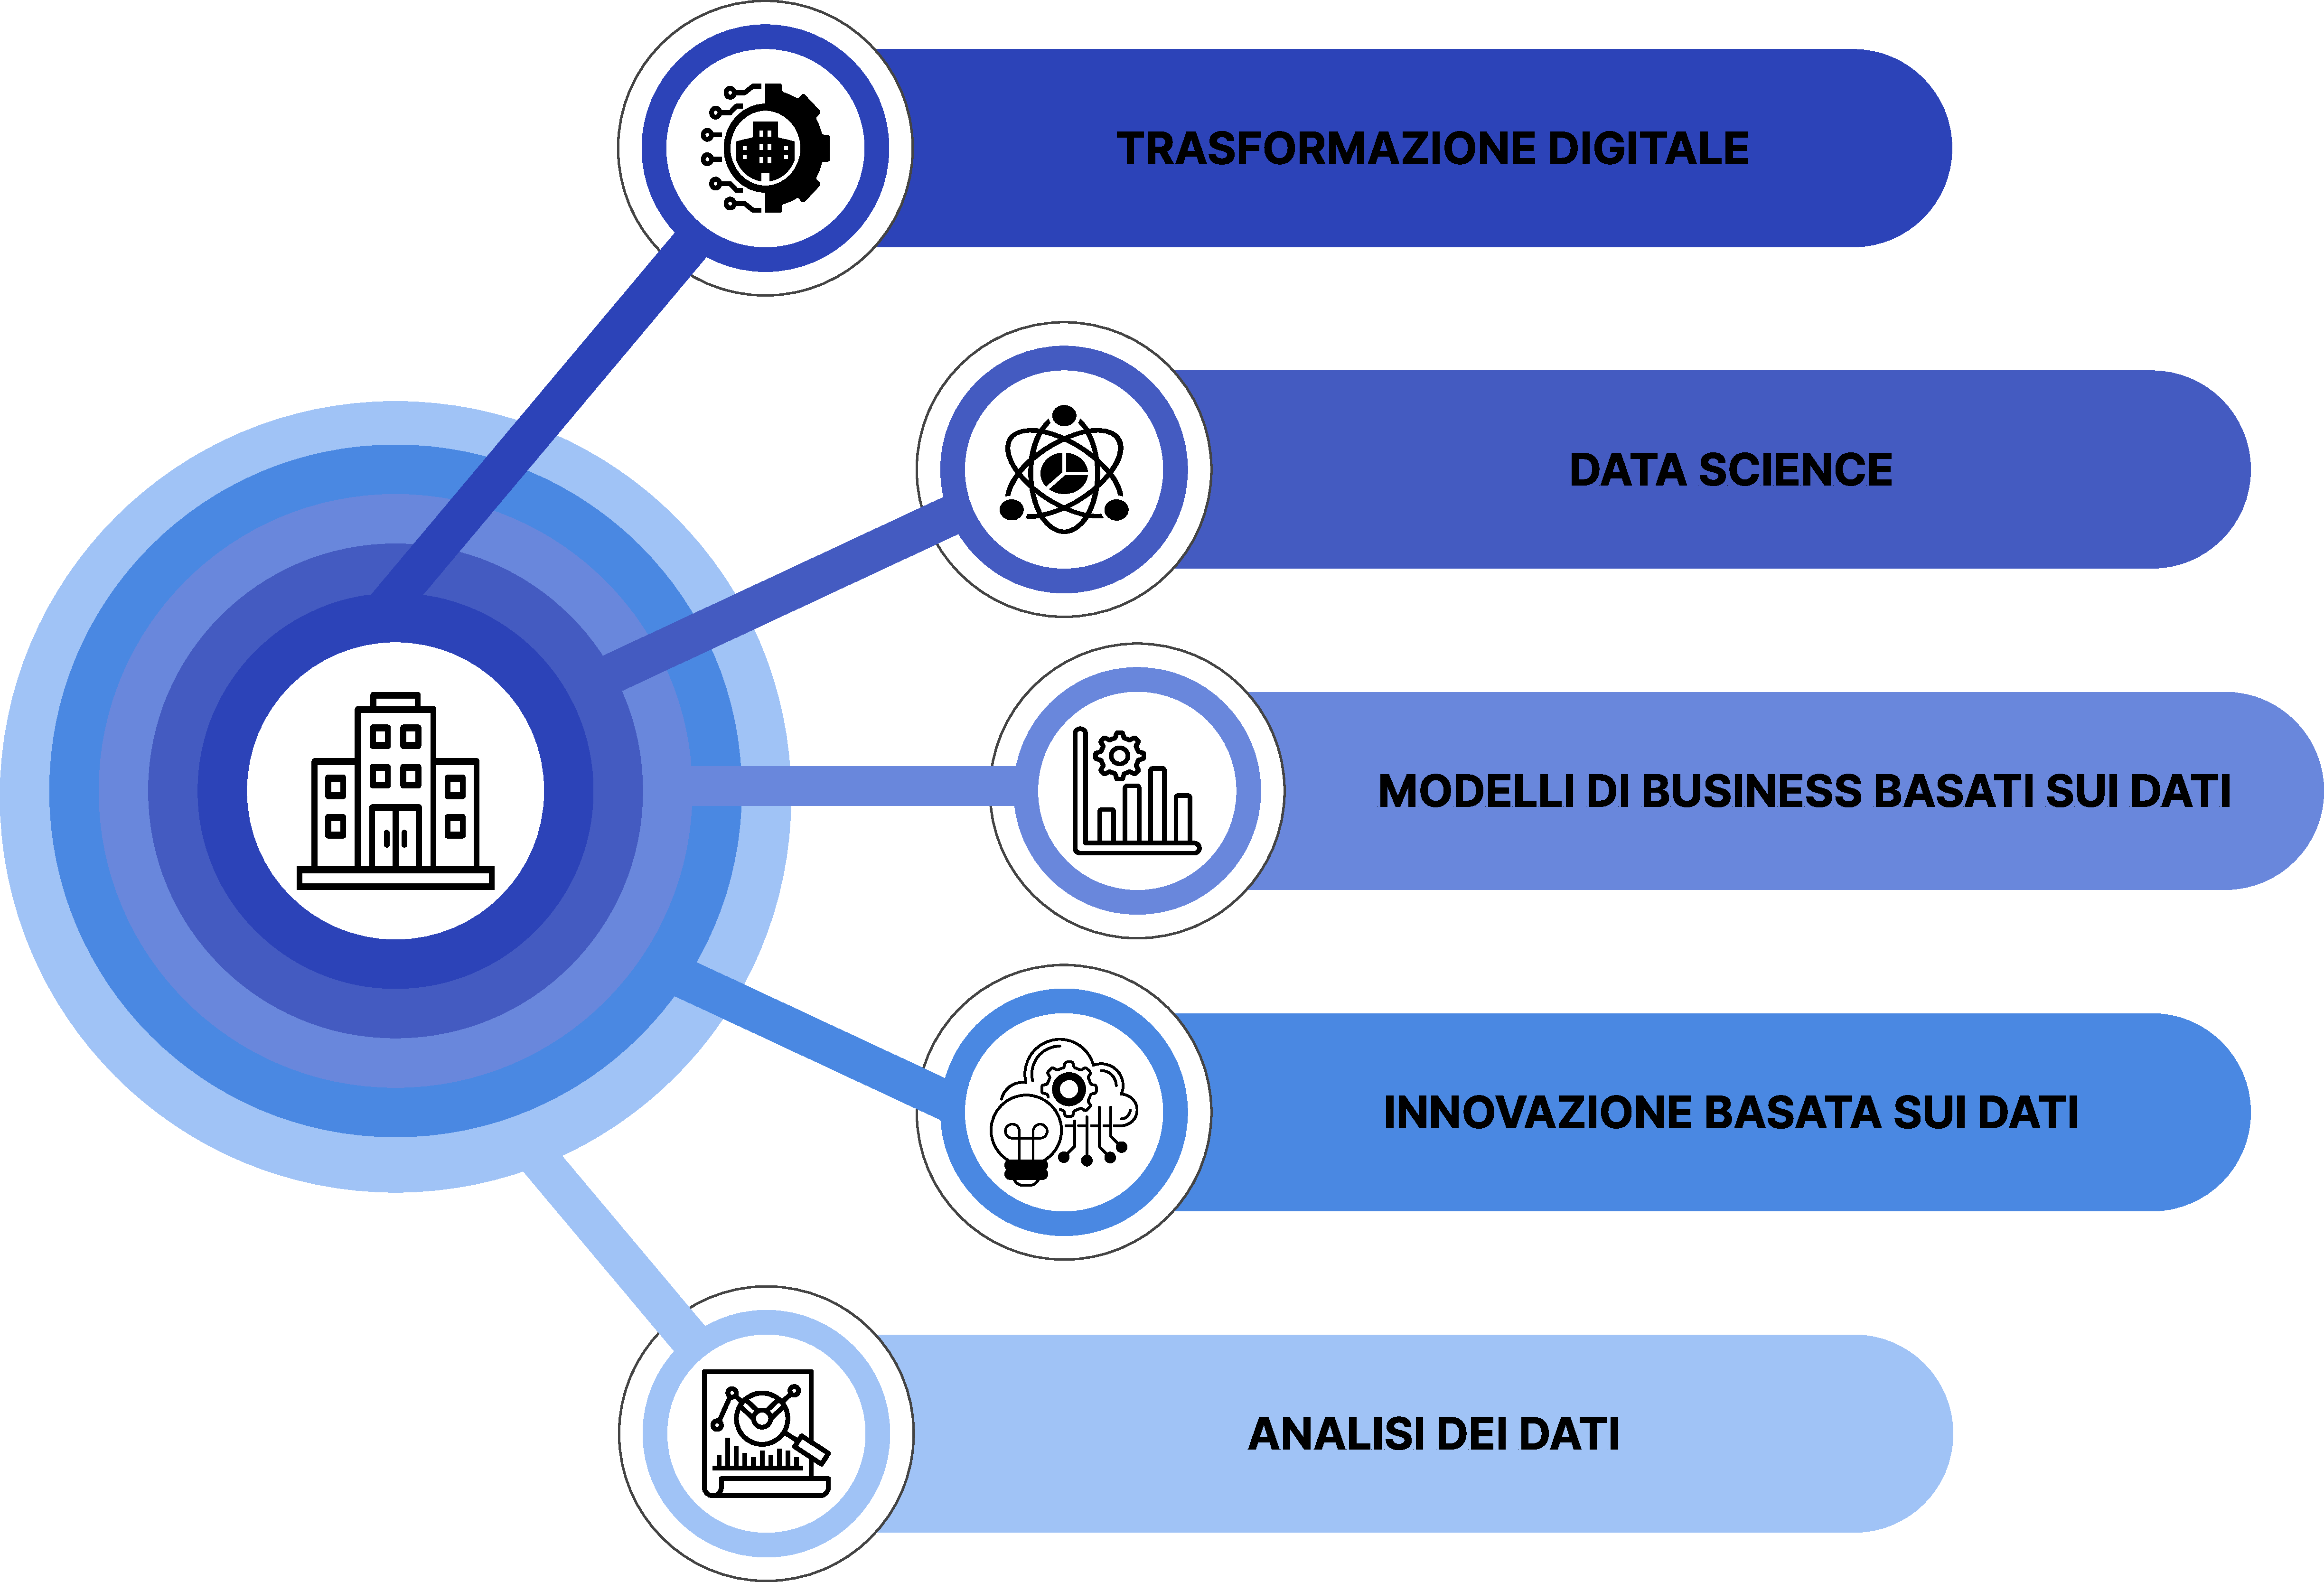
\includegraphics[width=0.75\linewidth]{figure/capitolo_1/Data-Driven company key points.pdf}
    \caption{Punti chiave delle aziende Data-Driven oriented}
    \label{fig:Data-Driven company key points}
\end{figure}

\section{Data Governance}
In un mondo come quello odierno in cui i dati sono uno degli asset di maggior valore, poterli gestire in modo efficace ed efficiente diventa fondamentale in qualsiasi ambito e a qualsiasi livello. Proprio per tale motivo l'Unione Europea ha presentato il documento \textit{Data Governance Act}\footnote{Il \textit{Data Governance Act} è una legge che mira a rendere disponibili più dati, regolando il riutilizzo di dati pubblici/protetti, incrementandone la condivisione dei dati attraverso una regolamentazione di nuovi intermediari di dati e incoraggiandone la condivisione a scopi altruistici.}.\cite{europe_data_governance_act}

La \textbf{governance dei dati} (\textit{Data Governance, DG}) promuove la disponibilità, la qualità e la sicurezza di questi all'interno di un'azienda attraverso diverse policy e standard. Questi processi determinano i proprietari, le misure di sicurezza e gli usi previsti per i dati. Nel complesso, l'obiettivo della DG è mantenere dati di alta qualità che siano sicuri e facilmente accessibili per ottenere informazioni aziendali più approfondite.\cite{ibm_data_governance}
Più precisamente, secondo la definizione di Gartner «La governance dei dati è la specificazione dei diritti decisionali e un quadro di responsabilità per garantire il comportamento appropriato nella valutazione, creazione, consumo e controllo dei dati e delle analisi».\cite{gartner_data_governance_definition}

\subsection{Domini della Data Governance}
Come espresso sopra, definire una governance dei dati all'interno di un'azienda permette di indicare chi detiene i diritti decisionali e le responsabilità riguardo gli asset dell'azienda in questione. Pertanto, è importante identificare quali sono i \textit{domini decisionali} di applicazione in modo da assegnare correttamente le responsabilità e i doveri alle persone: principi dei dati, qualità dei dati, metadati, accesso ai dati e ciclo di vita dei dati. I principi dei dati, che sanciscono i confini per l'uso degli asset dei dati che riguardano gli standard aziendali (andando in questo modo a stabilire la direzione per tutti gli altri domini decisionali); la qualità dei dati, che rifinisce la base per come i dati debbano essere interpretati (metadati) e siano accessibili agli utenti (accesso ai dati): infine, la decisione sul ciclo di vita dei dati definisce la loro produzione, conservazione e ritiro, svolgendo un ruolo fondamentale nell'operazionalizzare i principi dei dati nell'ambito delle infrastrutture IT.\cite{data_governance_activities}

\begin{figure}[!h]
    \centering
    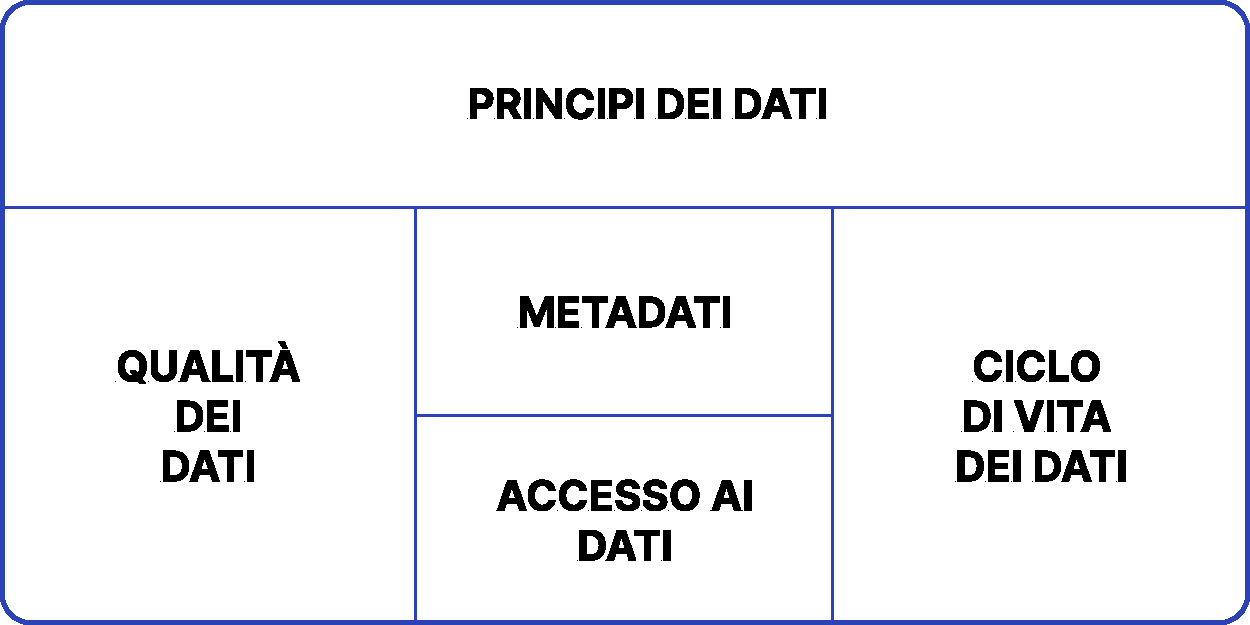
\includegraphics[width=0.75\linewidth]{figure/capitolo_1/Data Governance Dominions.pdf}
    \caption{Domini della Data Governance}
    \label{fig:Data Governance Dominions}
\end{figure}

\subsection{Vantaggi della governance dei dati}

Di seguito sono riportati i vantaggi che una corretta governance dei dati può comportare all'interno di un'azienda:\cite{google_data_governance}
\begin{itemize}
    \item Prendere decisioni migliori in minor tempo. I dipendenti di un'azienda acquisiscono i dati di cui necessitano per raggiungere e assistere i clienti, progettare e migliorare prodotti e servizi, sfruttando eventuali occasioni.
    \item Migliorare la gestione dei costi. I dati aiutano a gestire le risorse più efficacemente. Grazie ad una corretta gestione sarà inoltre possibile eliminare possibili duplicazioni dei dati, risparmiando spazio e soldi.
    \item Migliorare le conformità normative. Il costante cambiamento del mondo delle leggi e conformità da seguire rende ancora più importante per le organizzazioni una gestione solida e sicura in tale ambito, diminuendone i rischi.
    \item Guadagnare maggiore fiducia da parte dei clienti. La creazione di un sistema preciso, corretto, conforme e ben gestito permette alle aziende di avere un impatto più positivo e rassicurante agli occhi delle persone con cui deve interagire.
    \item Gestire i rischi in modo più semplice. Adoperando una governance corretta è possibile aumentare la sicurezza sull'esposizione dei dati sensibili a sistemi o individui che non dispongono di un'adeguata autorizzazione, sulla violazione della sicurezza da parte di malintenzionati.
    \item Consentire a più persone l'accesso ad una maggiore quantità di dati. Una governance ben strutturata permette ad un numero maggiore di utenti di accedere ai dati per loro necessari in minor tempo, avendo inoltre la certezza della correttezza degli stessi.
\end{itemize}

\section{Obiettivo della tesi}

\section{Struttura della tesi}
